\documentclass[a4paper,13pt]{scrartcl}
\usepackage[spanish]{babel}
\usepackage{hyperref}
\hypersetup{unicode=true, pdftex, colorlinks=true, linkcolor=blue, citecolor=blue, filecolor=blue, urlcolor=blue, pdftitle=RIOT Cast the First Stone - Spanish rules, pdfauthor=Ilario Gelmetti, pdfsubject=Riot Board Game}
\usepackage{graphicx}
\usepackage{tabularx}
\usepackage{geometry}

\geometry{
	top=0.85in,
	inner=1.2in,
	outer=1.2in,
	bottom=0.9in,
	headheight=2ex,
	headsep=2ex,
}
\setlength{\footskip}{30pt}



\renewcommand{\thesubsection}{\arabic{subsection}} % to remove the section numbers from subsections

\graphicspath{ {./img/} }

\title{RIOT Cast the First Stone}
\subtitle{Reglas del juego en Espa\~nol}
\author{}
\date{}
\begin{document}

\maketitle

Una versi\'on actualizada y corregida de las reglas puede ser encontrada en nuestra web:
\textbf{http://riotboardgame.com } 

Para correcciones escribir a Ilario Gelmetti \texttt{ilario@eigenlab.org}

\section*{Piezas}
1 tablero de juego - 42 cartas manifestantes - 10 cartas opini\'on publica - 2 cartas objetivo nacionalistas - 4
tableros jugadores - 96 piezas unidades

\section*{Tablero de juego}
El tablero de juego tiene una \textbf{Comisar\'ia} y en el interior de este un \textbf{Hospital}, luego hay \textbf{6 barrios} divididos por
l\'ineas blancas.

Cada barrio consta de: \textbf{edificios} (que pueden ser de 1 o de 2 cr\'editos), una calle y 2 \textbf{puntos de ingreso} (la
Comisar\'ia para la Polic\'ia y un marco redondo para los Manifestantes).

\section*{Bandos}
En RIOT hay 4 bandos: la \textbf{Polic\'ia} y 3 \textbf{Manifestantes}: Autonomen, Anarquistas y Nacionalistas.

\section*{Como se gana la partida}
\begin{itemize}
\item La \textbf{Polic\'ia} gana cuando se descubre la ultima Carta Opini\'on Publica.
\item Los \textbf{Autonomen} y los \textbf{Anarquistas} ganan cuando consiguen 7 Puntos Barrio.
\item Los \textbf{Nacionalistas} ganan cuando obtienen el objetivo secreto que s\'olo ellos conocen. Este objetivo se coge al
azar al principio de la partida.
\end{itemize}

\section*{Cartas Opini\'on Publica (Cartas OP)}
Una \textbf{carta Opini\'on Publica} se descubre \textbf{al final} de cada turno donde la \textbf{Polic\'ia} ha sido involucrada por lo menos en un
\textbf{enfrentamiento de contacto} que haya tenido un ganador (da igual si la Polic\'ia gana o pierde).

Al final del turno, si coge una carta OP, la Polic\'ia tambi\'en viene afectada por lo que la carta OP pone.

Cada turno puede ser descubierta \textbf{solo una carta OP}, si hay mas de un enfrentamiento de contacto igualmente la Polic\'ia
coge una sola carta por turno. Pero la Polic\'ia puede coger una carta OP tambi\'en en cada turno de los otros
jugadores si estos la atacan y hacen un enfrentamiento de contacto con ella, entonces en una partida con 4 jugadores la
Polic\'ia puede llegar a hacer un m\'aximo de 4 puntos por ronda.

\section*{Puntos Barrio}
Al principio de cada turno los Autonomen o los Anarquistas cogen un \textbf{Punto Barrio} por cada \textbf{barrio} donde tienen \textbf{ocupados
todos los edificios}.

\section*{Etapas del Turno}
\begin{enumerate}
\item Recuento de los Puntos Barrio y de los cr\'editos
\item Compra de Cartas y de Unidades
\item Posicionamiento de las Unidades
\item Movimiento y uso de las Cartas
\item Enfrentamientos
\end{enumerate}

\subsection{Recuento de los Puntos Barrio y de los
cr\'editos}
Autonomen y Anarquistas a principios de sus turnos miran los barrios donde controlan todos los edificio y apuntan
eventuales \textbf{Puntos Barrio} en su tabla de resumen.

Autonomen, Anarquistas y Nacionalistas cogen cr\'editos por cada edificio que controlan, cada edificio puede dar 1 o 2
cr\'editos, como pone el numero que est\'a pintado en el edificio mismo en el tablero de juego. Se puede poner mas
unidades en un edificio pero esto no sirve para cobrar m\'as cr\'editos.

La \textbf{Polic\'ia} calcula sus cr\'editos cada turno mirando a cuantas unidades enemigas hay en el juego, contando \textbf{solo las
del bando que tiene meno unidades}. Entonces la Polic\'ia cobra \textbf{un cr\'edito para cada unidad que hay de esto bando},
incluyendo las unidades heridas.

En la partida con \textbf{3 jugadores} la Polic\'ia cobra un \textbf{bonus de 2 cr\'editos} para cada turno.

En la partida con \textbf{4 jugadores} la Polic\'ia cobra un \textbf{bonus de 3 cr\'editos} para cada turno.

Los cr\'editos que no han sido utilizados se tiran, no pueden ser guardados para el turno siguiente.

\subsection{Compra de Cartas y de Unidades}
Con los cr\'editos obtenidos, cada bando puede \textbf{comprar cartas y unidades}. La \textbf{Polic\'ia} tiene \textbf{solo unidades} por comprar.

El precio de las unidades es indicado en la tabla de resumen de cada jugador.

Las \textbf{cartas tienen un precio que crece} si compras mas de una \textbf{en el mismo turno}: la primera que compras en un turno costa
1 cr\'edito, la segunda 2, la tercera 3, la cuarta 4. Entonces para comprar 3 cartas en el mismo turno se necesitan
1+2+3=6 cr\'editos.

\subsection{Posicionamiento de las Unidades}
Una vez que han sido compradas las unidades, el jugador \textbf{manifestante} las pone \textbf{en los Puntos de Ingreso} que prefiere. 

La \textbf{Polic\'ia} pone todas las unidades que compra \textbf{en la Comisaria}.

\subsection{Movimiento y uso de las Cartas}
\subsubsection*{Movimiento}
Despu\'es de haber posicionado las unidades en los Puntos de Ingreso, el jugador puede mover de \textbf{un movimiento cada una
de sus unidades}, incluidas las que acaba de crear y la que estaban heridas desde el turno anterior.

El primer movimiento de una unidad que acaba de ser creada y de las heridas es siempre \textbf{desde el Punto de Ingreso a la
calle del mismo barrio}. Les unidades \textbf{no se pueden quedar} en un Punto de Ingreso.

Las unidades que \textbf{ya est\'an en la calle} pueden \textbf{entrar en un edificio} vac\'io para ocuparlo o \textbf{atacar} un edificio que ya
est\'a ocupado. Pero para poder entrar o atacar un edificio se falta que en la calle no haya \textbf{ninguna unidad enemiga}, de
otra manera esta unidad puede decidir de \textbf{interponerse} o de dejar pasar. En caso que el jugador enemigo decida de
interponerse, el primero jugador puede decidir de usar algunas de sus unidades para atacar las que se interponen o
renunciar a entrar/atacar el edificio.

Las unidades pueden moverse libremente desde la calle de un barrio a la calle de un barrio cercano o salir de los
edificios sin que las unidades enemigas puedan interponerse.

Solo las unidades de la Polic\'ia pueden entrar en la Comisaria, desde la cual se puede llegar a todas las calles.

\subsubsection*{Cartas}
Las cartas pueden ser jugadas en \textbf{cualquier momento de tu turno} (antes, durante o despu\'es del movimiento), menos las
que son \textbf{cartas Blitz} (tienen el s\'imbolo de un rayo 
\includegraphics[height=9pt]{blitz.png}) que pueden ser usadas solo y siempre \textbf{en los enfrentamientos} donde
el jugador es involucrado.

\subsection{Enfrentamientos}
Todas las unidades pueden atacar a todos los grupos de unidades enemigas que se encuentran en un sitio donde puedan
alcanzar a llegar. Por ejemplo para \textbf{atacar un edificio} se falta tambi\'en \textbf{un movimiento}, como si las unidades que
atacan estuvieran entrando en este.

En un enfrentamiento se \textbf{suma la fuerza} de todas las unidades que atacan y se compara con la fuerza de las unidades que
defienden, quien tiene la fuerza mas grande gana, si hay un \textbf{empate} no pasa nada y \textbf{no se elimina} ninguna unidad.

Cada jugador tiene que declarar con cuales unidades est\'a atacando, puede elegir de atacar solo con algunas dejando las
otras listas para otras acciones. Al rev\'es, quien defiende, defiende siempre con todas las unidades que tiene en esta
\'area.

La Polic\'ia \textbf{no puede} nunca atacar cuando est\'a en \textbf{minor\'ia}.

Quien \textbf{defiende un edificio} recibe un \textbf{bonus de +1} a la fuerza en combate cuando los atacan. No se puede atacar desde un
edificio.

Un especifico grupo de unidades puede ser atacado m\'aximo dos veces por el mismo jugador en el mismo turno.

Los enfrentamientos se dividen en dos etapas: \textbf{enfrentamiento a distancia} y \textbf{enfrentamiento de contacto}.

Despu\'es de haber decidido cuales unidades atacan y el objetivo, empieza la etapa de enfrentamiento a distancia y los
dos jugadores pueden usar las \textbf{cartas Blitz de ataque a distancia} (ver mas abajo {\itshape ataques a distancia}). Cuando el
efecto de las cartas Blitz (
\includegraphics[height=9pt]{blitz.png}) ha sido aplicado, quien est\'a atacando \textbf{puede elegir} si seguir con el enfrentamiento de
contacto o \textbf{parar}.

Ahora los jugadores pueden jugar las \textbf{otras cartas Blitz} (las que no son de distancia) y luego se resuelve el
enfrentamiento calculando las \textbf{fuerzas} del atacante y del defensor.

El perdedor \textbf{elimina todas} las unidades involucradas de la plancha; el ganador \textbf{calcula su perdidas y sus heridos} (ver mas
abajo {\itshape perdidas y heridos}).

\subsubsection*{Ataques a distancia}
Cuando un jugador juega una carta Blitz de ataque a distancia en un enfrentamiento, de pronto \textbf{elige} cual de \textbf{las unidades
enemigas} defensores es el objetivo de esta carta. Esta unidad recibe \textbf{inmediatamente} el da\~no que pone la carta y se
\textbf{hiere} o se \textbf{saca del juego} (si el da\~no es suficiente), de todo modo no va a participar a la pr\'oxima fase del
enfrentamiento.

NB 1: Cada unidad de la Polic\'ia, excepto la mas b\'asica, \textbf{aguantan el primero punto de da\~no} de las cartas Blitz de
ataque a distancia, gracias a sus \textbf{escudos} (
\includegraphics[height=9pt]{shield.png}). Esto significa que contra estas unidades una carta de +1 es in\'util,
mientras una carta de +2 o dos de +1 juntas hacen un solo da\~no.

NB 2: si un enfrentamiento con la Polic\'ia se acaba en esta fase (por ejemplo si despu\'es de usar los ataque a
distancia hay un \textbf{empate} o la Polic\'ia es \textbf{en minor\'ia}) no hay \textbf{ning\'un efecto} en los puntos de \textbf{Opini\'on Publica}.

\subsubsection*{Perdidas y heridos}
El grupo de unidades ganador en un enfrentamiento recibe tantos \textbf{da\~nos} cuanto es la \textbf{fuerza del grupo perdedor}
involucrado. Los da\~nos se reparten empezando desde las unidades \textbf{mas d\'ebiles} (si la fuerza es igual, antes las mas
baratas). Una unidad est\'a \textbf{herida} si los da\~nos que recibe son \textbf{menos que su fuerza}.

Los Manifestantes ponen sus unidades heridas en el \textbf{punto de ingreso} del barrio donde ha pasado el enfrentamiento; al
pr\'oximo turno estas unidades son \textbf{como nuevas} y pueden mover en la calle otra vez.

La Polic\'ia pone sus unidades heridas en el \textbf{Hospital}; estas pueden \textbf{mover en la Comisaria} al turno siguiente y, en otro
turno mas, salir a la calle como si fueran nuevas.

\subsubsection*{Atacar y defender un edificio}
Las unidades en un edificio tienen un \textbf{bonus de +1 a la fuerza} para defender. Desde dentro el edificio \textbf{no pueden atacar}.

Quien ataca \textbf{no puede usar cartas Blitz} de ataque a distancia en contra de unidades en un edificio, pero \textbf{el defensor
puede} usarlas.

Si el atacante gana, todas sus unidades que \textbf{sobreviven} (incluidas las heridas por el enfrentamiento de contacto) \textbf{entran}
ya a ocupar el edificio (menos si es la Polic\'ia, que no entra nunca en los edificios).

Si el defensor gana, todas sus unidades que sobreviven (incluidas las heridas) \textbf{se quedan} en el edificio.

\section*{Primera ronda}
Cada jugador Manifestante, siguiendo un orden aleatorio, pone una unidad \textbf{de las mas b\'asicas} que tiene en el interior
de un edificio, uno cualquier. Cada jugador pone \textbf{otra unidad b\'asica} hasta cuando cada jugador tenga \textbf{dos edificios} ocupados con
una unidad cada uno en \textbf{dos barrios distintos}.

\textbf{Partida con 2 jugadores:} El Manifestante pone \textbf{3 unidades} en 3 edificios de 3 barrios distintos.

Ahora la Polic\'ia cobra los cr\'editos y puede empezar su primero turno.

Desde ahora, la Polic\'ia, al final de cada turno suyo, \textbf{elige el orden} de los turnos de los otros jugadores.

\section*{Unidades especiales}
\begin{minipage}[c]{0.2\textwidth}
\centering
\textbf{Mediactivista}
\smallskip


\includegraphics[width=2cm]{special_units-mediaactivist.png}
\end{minipage}\hfill
\begin{minipage}[c]{0.75\textwidth}

\includegraphics[width=1cm]{po.png} Cuando esta unidad es involucrada en un enfrentamiento con la Polic\'ia, este enfrentamiento no
vale para los puntos de Opini\'on Publica. 
\smallskip


\includegraphics[width=1cm]{card.png} Cuando esta unidad est\'a defendiendo y se elimina, el jugador coge una carta por gratis.
\end{minipage}
\bigskip

\begin{minipage}[c]{0.2\textwidth}
	\centering
	\textbf{Black Block}
	\smallskip
	
	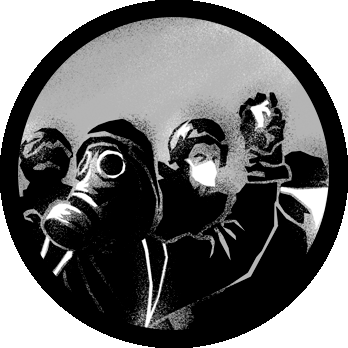
\includegraphics[width=2cm]{special_units-blackblock.png}
\end{minipage}\hfill
\begin{minipage}[c]{0.75\textwidth}
	
\includegraphics[width=1cm]{street.png} Cuando ataca alguien en la calle desde la calle tiene fuerza 3, de otra manera (si defiende o
	ataca un edificio) tiene fuerza 2.
\end{minipage}
\bigskip

\begin{minipage}[c]{0.2\textwidth}
	\centering
	\textbf{Paramilitar}
	\smallskip
	
	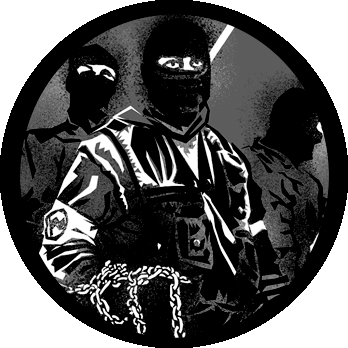
\includegraphics[width=2cm]{special_units-paramilitar.png}
\end{minipage}\hfill
\begin{minipage}[c]{0.75\textwidth}
	
\includegraphics[width=1cm]{direct_enter.png} En el primero turno cuando acaba de ser creada, esta unidad puede atacar directamente (siempre que
en la misma calle no haya nadie a pararla) un edificio ocupado. No puede entrar directamente en un edificio vac\'io, solo atacar uno ocupado.
\end{minipage}
\bigskip

\begin{minipage}[c]{0.2\textwidth}
	\centering
	\textbf{Camioneta}
	\smallskip
	
	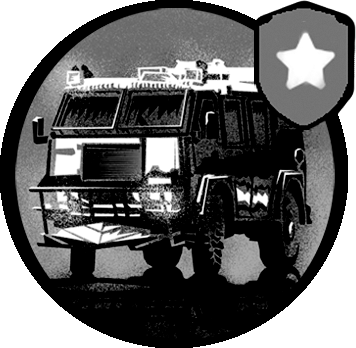
\includegraphics[width=2cm]{special_units-van.png}
\end{minipage}\hfill
\begin{minipage}[c]{0.75\textwidth}
	
\includegraphics[width=1cm]{movement.png} Puede mover de dos movimientos cada turno, tambi\'en para salir de el Hospital.
\end{minipage}
\bigskip

\begin{minipage}[c]{0.2\textwidth}
	\centering
	\textbf{SWAT}
	\smallskip
	
	
\includegraphics[width=2cm]{special_units-swat.png}
\end{minipage}\hfill
\begin{minipage}[c]{0.75\textwidth}
	
\includegraphics[width=1cm]{direct_enter.png} En el primero turno cuando acaba de ser creada, esta unidad puede atacar directamente (siempre que en la
misma calle no haya nadie a pararla) un edificio ocupado.
\end{minipage}

\section*{Preguntas frecuentes}
{\bfseries
?`Cuantas unidades pueden estar en un edificio al mismo tiempo?} \nopagebreak

No hay l\'imite. De toda manera, no se cobra m\'as fichas de cr\'edito por tener m\'as unidades en un edificio. A veces,
merece la pena poner m\'as unidades en cada edificio para proteger mejor el barrio.
\bigskip

{\bfseries
?`Qu\'e pasa si en un enfrentamiento donde participa tambi\'en la Polic\'ia se resuelve con los ataques a distancia
(entonces no hay enfrentamiento de contacto)?} \nopagebreak

La Polic\'ia no recibe ning\'un punto porque no se ha tenido alg\'un enfrentamiento de contacto (entonces no gira
ninguna carta Opini\'on P\'ublica).
\bigskip

{\bfseries
?`Como funciona la carta ``+1 pero m\'aximo empate''?} \nopagebreak

El jugador Autonomen puede usar esta carta para perder haciendo m\'as da\~no, o para llegar a un empate (entonces no
pasa nada).
\bigskip

{\bfseries
?`Como evito la victoria de la Polic\'ia?} \nopagebreak

Si no tienes ninguna carta o unidad que te permita de atacar la Polic\'ia sin que esta coja una carta de Punto Opini\'on
P\'ublica, intenta de no hacerlo.

Recuerda que la Polic\'ia puede hacer un Punto Opini\'on P\'ublica para cada turno cuando participa en un enfrentamiento
(que no se acabe con la fase de ataque a distancia y que no sea un empate) entonces podr\'ia llegar a hacer mas de un
punto por cada ronda si los otros jugadores la atacan.

Los Autonomen pueden ser mas tranquilos con las unidades mediactivista que si es presente en el enfrentamiento hace que
la Polic\'ia no coja una carta de Opini\'on P\'ublica.

Los Anarquista pueden comprar muchas cartas para tener cartas ``Ning\'un efecto su Opini\'on Publica''.

Los Nacionalistas tendr\'ian que no atacar nunca la Polic\'ia, y cuando esta los ataca pueden usar la carta ``No
enfrentamiento''.
\bigskip

{\bfseries
?`Si alguien se interpone en un enfrentamiento declarado, que pasa?} \nopagebreak

Quien ataca puede elegir con cuales unidades atacar. Despu\'es de que estas unidades hayan sido heridas o eliminadas, el
atacante podr\'a seguir el ataque con otras unidades que todav\'ia no haya usado.
\bigskip

{\bfseries
?`Tengo que hacer salir las unidades que est\'an en un punto de ingreso (unidades que acabo de crear o que han sido
heridas a la ronda anterior)?} \nopagebreak

S\'i, esto vale para todos, la Polic\'ia y los Protestantes. La \'unica diferencia es que las unidades de la Polic\'ia,
despu\'es de haber salido de el Hospital, pueden quedarse en la Comisaria cuanto quieran.
\bigskip

{\bfseries
?`Qu\'e pasa si una unidad viene herida atacando un edificio?} \nopagebreak

Si gana el ataque, entra igualmente en el edificio (juntas con las que no han sido heridas) y no pierde los puntos de
vida.
\bigskip

{\bfseries
?`Qu\'e significa ``ataque combo''?} \nopagebreak

Si quieres entrar en (o atacar) un edificio con unidades que tienes en la calle, pero en la misma calle hay enemigos,
estos pueden decidir de no dejarte pasar. En el caso que suceda, puedes intentar un ataque combo. Significa sacar las
unidades del enemigo de la calle usando unidades nuevas que acabas de crear y luego entrar en (o atacar) el edificio
con las unidades que ya ten\'ias en la calle y que no has usado para atacar (y que entonces todav\'ia no han usado su
movimiento).

Acuerda de girar las unidades que has usado para el ataque para distinguirlas desde las otras.
\bigskip

{\bfseries
?`Qu\'e pasa si una unidad resulta herida defendiendo un edificio?} \nopagebreak

Se queda en el edificio, sin perder ning\'un punto de vida.
\bigskip

{\bfseries
?`Qu\'e pasa si en un enfrentamiento, despu\'es de usar las cartas (por ejemplo las de ataque a distancia), acaba en
empate?} \nopagebreak

Si el enfrentamiento acaba en empate ninguna unidad viene eliminada y las unidades del atacante no pueden tener m\'as
movimientos.
\bigskip

{\bfseries
?`La Polic\'ia puede entrar en los edificios?} \nopagebreak

No, puede entrar y salir \'unicamente desde la Comisaria de Polic\'ia y el Hospital que tiene al interior. Tampoco
pueden entrar aunque hayan ganado atacando un edificio: las unidades de la Polic\'ia que no est\'an muertas ni heridas
se quedan en la calle (y terminan sus movimientos).
\bigskip

{\bfseries
?`Qu\'e bandos tengo que usar en una partida con dos jugadores?} \nopagebreak

El juego ha sido probado jugando con Polic\'ia y Aut\'onomos. La Polic\'ia no coge cr\'editos bonus (como pasa en la
partida a 3 y 4 jugadores). De toda manera pod\'eis probar combinaciones diferentes si quer\'eis.
\bigskip

{\bfseries
?`Qu\'e bandos tengo que usar en una partida con tres jugadores?} \nopagebreak

El juego ha sido probado jugando con \ Polic\'ia y Aut\'onomos y Anarquistas. La Polic\'ia coge un bonus de 2 cr\'editos
cada turno. De toda manera pod\'eis probar combinaciones diferentes si quer\'eis.
\bigskip

{\bfseries
?`Por qu\'e las unidades tienen dos caras?} \nopagebreak

Para ayudarte a recordar cuales ya han completado su acci\'on y cuales se pueden todav\'ia usar.
\bigskip

{\bfseries
?`Puede pasar que un jugador sea eliminado desde el juego?} \nopagebreak

S\'i, pasa cuando un jugador manifestante no tiene m\'as unidades. Esto no vale para la Polic\'ia, que sigue jugando tambi\'en si no tiene m\'as unidades.
\bigskip

{\bfseries
?`Cada unidad puede atacar una vez por cada ronda o cada turno?} \nopagebreak

Cada jugador puede usar sus unidades para mover y/o atacar solo en su turno, entonces solo una vez por cada ronda, pero
estas unidades pueden defender todas las veces que alguien las ataca.
\bigskip

{\bfseries
?`Las unidades que atacan un edificio pueden ``morir''?} \nopagebreak

Claramente s\'i, las que sean eliminadas se sacaran del juego. Si los atacantes ganan, las unidades heridas juntas con
las no heridas entran directamente en el edificio ocup\'andolo.
\bigskip

{\bfseries
?`Si una mediactivista que se interpone en un enfrentamiento y es eliminada, el jugador Autonomen coge su carta?} \nopagebreak

S\'i, es como si la mediactivista estuviera defendiendo.
\bigskip

{\bfseries
?`Pueden entrar unidades de grupos diferentes desde el mismo punto de ingreso?} \nopagebreak

Claramente s\'i!

\section*{Glosario}
\textbf{Protestantes}:\textbf{ }todos los bandos excepto la Polic\'ia.

\textbf{Tablero}: representa una peque\~na ciudad con 6 \'areas y una Comisaria de la Polic\'ia en el medio.

\textbf{Cr\'editos}: puedes usarlos para comprar Cartas Riot o para crear unidades.

\textbf{Cartas Riot}: \'unicamente los Protestantes pueden tener Cartas Riot, dan varios bonus y las puedes utilizar
durante tu turno.

\textbf{Cartas Riot Blitz}: puedes utilizar \'unicamente durante un enfrentamiento donde estas involucrado directamente.
Tienen un rel\'ampago (
\includegraphics[height=9pt]{blitz.png}) pintado su la carta.

\textbf{Cartas Opini\'on P\'ublica}: son los puntos de victoria para la Polic\'ia, pero tambi\'en hacen da\~no a la
Polic\'ia cada vez que se gira una.

\textbf{Ocupaci\'on}: cuando una o mas unidades de los Protestantes entran en un edificio.

\textbf{Desalojo}: cuando unas unidades atacan un edificio ocupado.

\textbf{Movimiento}: cuando un jugador cambia de sitio una unidad desde un Punto de Ingreso hasta una calle, desde una
calle hasta una otra adyacente, desde una calle hasta dentro un edificio en la misma calle y el rev\'es. 

\textbf{Punto de Ingreso}: en cada calle hay un circulo blanco donde las unidades aparecen cuando acaban de ser creadas.
Para salir a la calle se necesita un movimiento.

\textbf{Enfrentamiento}: cuando un jugador elige unas de sus unidades para atacar todas las unidades de un enemigo en
una \'area (una calle o un edificio). Puedes atacar solo donde puedes moverte (entonces para atacar un edificio, tus
unidades necesitan tambi\'en un movimiento).

\textbf{Interposici\'on}: cuando un jugador decide de usar todas sus unidades en una area para ponerse en el medio de un
ataque que acaba de ser declarado en la misma calle. El jugador que ha declarado el ataque puede dejar o atacar las
unidades que se han puesto en el medio.

\textbf{Ataque a distancia}: las Cartas Riot Blitz (
\includegraphics[height=9pt]{blitz.png}) hacen da\~no al enemigo antes del contacto, cada Carta Riot Blitz
tiene que ser dirigida a una unidad y mas cartas pueden ser dirigidas contra la misma unidad, agregando el da\~no.
Pueden ser usada sea defendiendo que atacando, pero no atacando un edificio.

\textbf{Puntos de barrio}: los Autonomen y los Anarquista cogen puntos de barrio al principio de cada propio turno, uno
por cada barrio donde ocupan todos los edificios.

\textbf{Objetivo secreto}: los Nacionalistas tienen un objetivo secreto para ganar el partido, esto lo cogen al azar al
principio del partido sin ense\~narlo a los dem\'as.

\textbf{Turno/Ronda}: un Turno es lo que juega un solo jugador, una Ronda es la suma de un Turno por cada jugador.
\end{document}